\documentclass[screen, aspectratio=169]{beamer}
\usepackage[T1]{fontenc}
\usepackage[utf8]{inputenc}
\usepackage{tikz, environ, listings}

% Use the NTNU-temaet for beamer 
% \usetheme[style=ntnu|simple|vertical|horizontal, 
%     language=bm|nn|en, 
%     smalltitle, 
%     city=all|trondheim|alesund|gjovik]{ntnu2017}
\usetheme[style=horizontal,language=bm]{ntnu2015}

\usepackage[norsk]{babel}

\title[Short title]{Øvingsforelesning 3 Python (TDT4110)}
\subtitle{For og While-løkker}
\author[O.M. Pedersen]{Ole-Magnus Pedersen}
\institute[NTNU]{}
\date{}
%\date{} % To have an empty date

\NewEnviron{transparent}{
	\tikz\node[opacity=0.2,align=left,inner xsep=0]{\parbox[t]{\linewidth}{
			\BODY
		}};
	}

\hypersetup{
	colorlinks,
	urlcolor={blue!70!black}
}

\RequirePackage{listings, color, textcomp}
\lstset{
	tabsize=2,
	rulecolor=,
	basicstyle=\ttfamily\small,
	upquote=true,
	aboveskip={1.5\baselineskip},
	columns=fixed,
	showstringspaces=false,
	extendedchars=true,
	literate={æ}{{\ae}}1
			 {ø}{{{\o}}}1
			 {å}{{\aa}}1
			 {Æ}{{\AE}}1
			 {Ø}{{\O}}1
			 {Å}{{\AA}}1,
	breaklines=true,
	breakatwhitespace=true,
	escapeinside={(*}{*)},
	showtabs=false,
	showspaces=false,
	keepspaces=true,
	showstringspaces=false,
	frame=l,
	identifierstyle=\ttfamily,
	keywordstyle=\color[rgb]{1.0,0,0},
	keywordstyle=[1]\color[rgb]{0,0,0.75},
	%keywordstyle=[2]\color[rgb]{0.5,0.0,0.0},
	keywordstyle=[3]\color[rgb]{0.127,0.427,0.514},
	keywordstyle=[4]\color[rgb]{0.4,0.4,0.4},
	commentstyle=\color[rgb]{0.133,0.545,0.133},
	stringstyle=\color[rgb]{0.639,0.082,0.082},
	mathescape
}
\lstset{language=Python}

\definecolor{secondaryColor}{RGB}{121, 162, 206}

\usetikzlibrary{shapes.geometric,arrows, positioning, calc}
\tikzstyle{process} = [rectangle, minimum width=2cm, minimum height=1cm, text centered, draw=black, fill=secondaryColor]
\tikzstyle{decision} = [diamond, minimum width=2cm, minimum height=1cm, text centered, draw=black, fill=secondaryColor]

\begin{document}

\begin{frame}
  \titlepage
\end{frame}

% Alternatively, special title page command to get a different background
% \ntnutitlepage

\begin{frame}{Oversikt}
	\begin{itemize}
		\item Praktisk Info
		\begin{transparent}
			\item Gjennomgang av øving 1
			\item Programmering for Øving 3
		\end{transparent}
	\end{itemize}
\end{frame}

\begin{frame}{Studasser og Piazza}
	\begin{itemize}
		\item Studasser er der for å hjelpe
		\begin{itemize}
			\item Bruk andre studasser dersom din har lang kø
		\end{itemize}
		\vspace{1em}
		\item Piazza er et godt sted å stille spørsmål
		\begin{itemize}
			\item \href{piazza.com/ntnu.no/fall2017/tdt4110}{piazza.com/ntnu.no/fall2017/tdt4110}
		\end{itemize}
	\end{itemize}
\end{frame}

\begin{frame}[fragile]{Kahoot!}
	\begin{itemize}
		\item Tilbakemelding på øvingsopplegget
		\item Sjekke ut mulighet for å redusere til to paralleller
		\tiny \item \href{https://play.kahoot.it/#/k/09d6073f-6747-4f20-ac5d-ffdd2bbb8911}{Link}
	\end{itemize}
\end{frame}

\begin{frame}{Oversikt}
	\begin{itemize}
		\begin{transparent}
			\item Praktisk informasjon
		\end{transparent}
		\item Gjennomgang av Øving 1
		\begin{transparent}
			\item Programmering for Øving 3
		\end{transparent}
	\end{itemize}
\end{frame}

\begin{frame}{Oversikt}
	\begin{itemize}
		\begin{transparent}
			\item Praktisk informasjon
			\item Gjennomgang av Øving 1
		\end{transparent}
		\item Programmering for Øving 3
	\end{itemize}
\end{frame}

\begin{frame}{Løkker}
	\begin{columns}
		\begin{column}{.4\textwidth}
			\begin{itemize}
				\item Brukes dersom deler av programmet skal kjøres flere ganger
				\item Om den kjøres igjen kontrolleres av en betingelse
			\end{itemize}
		\end{column}
		\begin{column}{.6\textwidth}
			\raggedright
			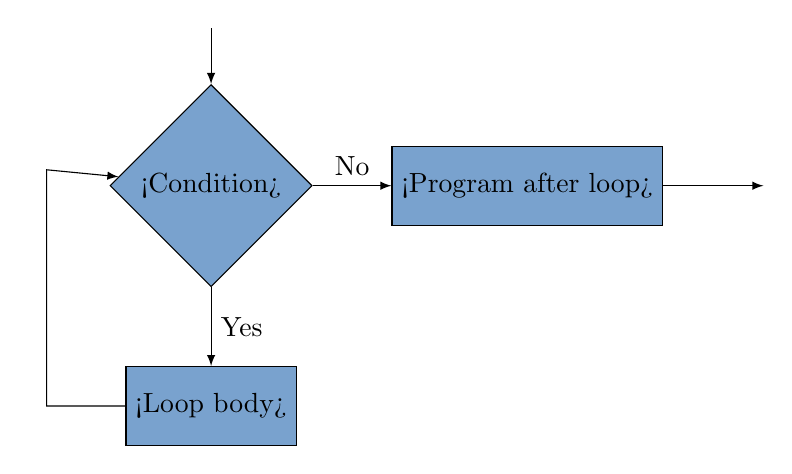
\begin{tikzpicture}
				\node (dec) [decision] {<Condition>};
				\node (body) [process, below=of dec] {<Loop body>};
				\node (exit) [process, right=of dec] {<Program after loop>};
				\node (botanchor) [left=of body]{};
				
				\draw[-latex] (0, 2) -- (dec);
				\draw[-latex] (dec) -- node[anchor=west]{Yes} (body);
				\draw[-latex] (dec) -- node[anchor=south]{No} (exit);
				\draw[-latex] (exit) -- ($(exit) + (3,0)$);
				\draw[-latex] (body) -- (botanchor.east) -- ($(botanchor.east) + (0, 3)$) -- (dec);
			\end{tikzpicture}
		\end{column}
	\end{columns}
\end{frame}

\begin{frame}[fragile]{for-løkker}
	\begin{itemize}
		\item Kjører koden et gitt antall ganger
		\item Antall ganger den skal kjøres må vites før man løkken starter
		\item Teknisk sett går den gjennom elementene i en \lstinline|iterable|
	\end{itemize}
	\vspace{-1em}
	\begin{lstlisting}
for i in range(100):
	print(i) # Printer tallene fra 0 til 99
for j in range(5, 10):
	print(j) # Printer tallene fra 5 til 9
for k in range(0, 20, 2):
	print(k) # Printer partall fra 0 til 19
	
for karakter in "dette er en streng":
	print(karakter) # Printer hver bokstav i strengen
for num in [1, 4, 6, 7]:
	print(num) # Printer hvert tall i lista
	\end{lstlisting}
\end{frame}

\begin{frame}{Eksempel}
	\begin{itemize}
		\item Skriv et program som summerer sammen tallene fra 4 til 20 (inklusiv)
	\end{itemize}
\end{frame}

\begin{frame}{Oppgave}
	\begin{itemize}
		\item Lag et program som tar inn to tall fra brukeren, og skriver ut alle tallene mellom disse (første inklusiv, andre eksklusiv) som er delelig på 3
	\end{itemize}
\end{frame}

\begin{frame}[fragile]{while-løkke}
	\begin{itemize}
		\item Løkken kjører så lenge en betingelse er oppfylt
	\end{itemize}
	\begin{lstlisting}
while <condition>:
	# Code to perform in loop

while password != real_password:
	password = input("Feil passord, prøv igjen: ")
	\end{lstlisting}
\end{frame}

\begin{frame}{Eksempel}
	\begin{itemize}
		\item Skriv et program som tar inn et tall og summerer tallene fra 1 og oppover helt til summen overstiger det oppgitte tallet. Skriv ut hvert regnestykke til konsollen.
	\end{itemize}
\end{frame}

\begin{frame}{Oppgave}
	\begin{itemize}
		\item Lag en while-løkke som skriver ut alle tallene fra 10 til og med 0.
	\end{itemize}
\end{frame}

\begin{frame}{Oppgave}
	\begin{itemize}
		\item Lag et program som tar inn et tall fra brukeren og sjekker om det er likt et annet tall du har bestemt på forhånd. Hvis tallene ikke er like, skal programmet si om det innskrevne tallet er større eller mindre enn målet, og brukeren skal få gjette igjen.
		\item Om tallet er riktig skal programmet si ifra om dette og avslutte.
	\end{itemize}
\end{frame}

\begin{frame}[fragile]{Break og continue}
	\begin{itemize}
		\item Noen ganger vil man avslutte løkken før den egentlig er ferdig
		\begin{itemize}
			\item Man har funnet det man leter etter
			\item Man er ferdig med en oppgave
			\item Bruker velger å avslutte
		\end{itemize}
		\item \lstinline|break| lar oss avslutte
		\item Andre ganger vil man avslutte en runde i løkken (men så starte på en ny):
		\begin{itemize}
			\item Ugyldig input fra bruker
			\item Operasjoner som bare skal gjøres i spesifikke iterasjoner (f.eks. partall)
		\end{itemize}
		\item \lstinline|continue| lar oss gjøre dette
	\end{itemize}
\end{frame}

\begin{frame}[fragile]{Else}
	\begin{itemize}
		\item Kode i \lstinline|else|-blokken kjøres bare hvis loopen ikke ble avsluttet ved et break
	\end{itemize}
	\begin{lstlisting}
for i in range(n):
	if i % k == 0:
		break
	<do stuff>
else:
	<do stuff if break was never reached>
	\end{lstlisting}
\end{frame}

\begin{frame}{Oppgave}
	\begin{itemize}
		\item<1-> Skriv en while-løkke som tar inn et tall hver iterasjon og summerer tallene
		\begin{itemize}
			\item Hint: \lstinline|while True:|
		\end{itemize}
		\item<2-> Gjør at programmet avsluttes dersom $-1$ skrives inn (uten å legge -1 til i summen)
		\item<3-> Avslutt programmet dersom summen går over 100 (men skriv ut siste summen)
	\end{itemize}
\end{frame}

\begin{frame}{Oppgave}
	\begin{itemize}
		\item Lag et program som tar inn en tekststreng fra brukeren. For hver karakter i strengen skal programme sjekke om det er et tall, og hvis det er det skal det legges til i en sum. Til slutt skal summen skrives ut.
		\begin{itemize}
			\item \lstinline|str.isnumeric(), int(str)|
		\end{itemize}
	\end{itemize}
\end{frame}

\begin{frame}{Oppgave}
	\begin{itemize}
		\item<+-> Lag et program som printer 10 tilfeldige tall
		\begin{itemize}
			\item \lstinline|import random, random.randint(min, max)|
		\end{itemize}
		\item<+-> Modifiser programmet til å også printe ut hvor mange oddetall som ble laget
		\item<+-> Print også ut det høyeste tallet som ble laget
	\end{itemize}
\end{frame}

\begin{frame}{Oppgave}
	\begin{itemize}
		\item<+-> Lag et program som tar inn to heltall fra brukeren, max og target. Programmet skal generere tilfeldige tall mellom 0 og max helt til det lager target, og printe hvert tall.
		\item<+-> Utvid programmet til å til slutt printe ut hvor mange forsøk det trengte for å lage target
	\end{itemize}
\end{frame}

\begin{frame}{Spørsmål}
	\begin{itemize}
		\item Spørsmål og tilbakemeldinger til øvingsforelesningene kan sendes til \href{mailto::olemagnp@stud.ntnu.no}{olemagnp@stud.ntnu.no}
	\end{itemize}
\end{frame}

\end{document}